\subsection{Mantle convection}\label{sec:mantle}
This problem is performed as presented by \citet{Blankenbach1989} (constant viscosity cases) and \citet{Thieulot2014}, in a 2D unit square domain with gravity
acceleration $g_y=10^{10}Ra$. The experiment is performed with three different Rayleigh numbers ($Ra=10^4$, $10^5$ and $10^6$) and with different grid
resolution (between $32\times32$ and $128\times128$ elements). The fluid has constant viscosity, initial density, heat capacity, thermal conductivity
($\eta= \rho_0= C_p = k=1$), reference temperature ($T_0=0$) and thermal expansion coefficient ($\alpha=10^{-10}$). Temperatures are set to 0 on top and 1 on
bottom of the domain. Velocity boundary conditions are set to free slip on all sides. The initial temperature field is given by
\[T(x,y)=(1-y)+0.01 \cos (\pi x) \sin (\pi y)\]

The solution generated by the code in terms of $v_{\textrm{rms}}$ (calculated as in Sec. \ref{sec:error}) and Nu as function of time are reported for all the
simulations in Fig. \ref{fig:mantle}. At the steady state, $v_{\textrm{rms}}$ and Nu of all simulations converge well toward the values from \citet{Blankenbach1989},
with lower errors for higher resolution grids (Table \ref{tab:mantle}). All data can be found at 
\url{https://github.com/aleregorda/Benchmarks/tree/main/Momentum%2BEnergy/Mantle_convection}.

\begin{figure}
\centering
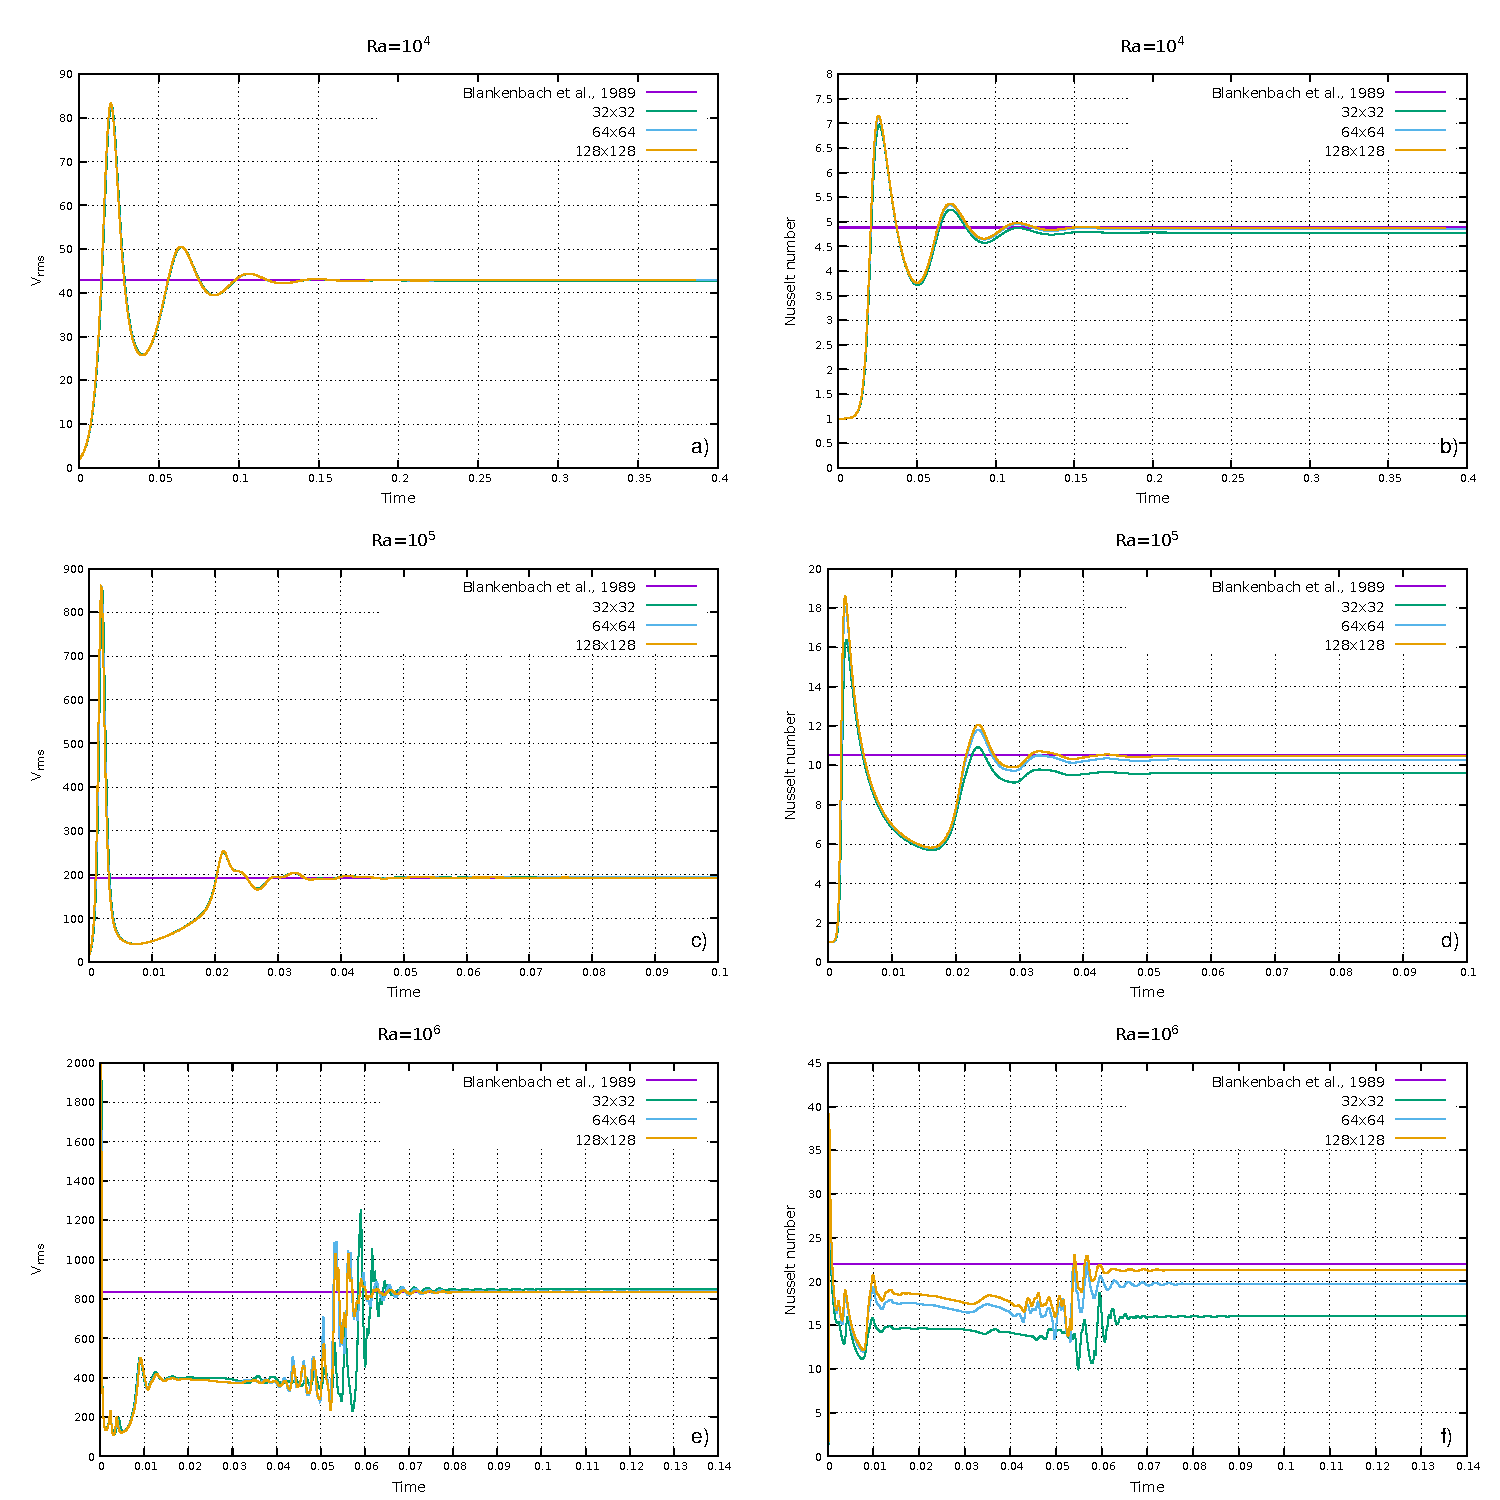
\includegraphics[width=400px]{./Figures/Convection.pdf}
\caption{$v_{\textrm{rms}}$ (panels a, c and e) and Nu (panels b, d and f) for the mantle convection benchmark as function of time for different grid resolution.
Panels a and b show the results for $Ra=10^4$; Panels c and d show the results for $Ra=10^5$; panels e and f show the results for $Ra=10^6$. Purple lines
indicate the convergence values for the $v_{\textrm{rms}}$ and the Nu from \citet{Blankenbach1989} at the steady state.}
\label{fig:mantle}
\end{figure}

\begin{table}[H]
\caption{Comparison between $v_{\textrm{rms}}$ and Nu predicted by the code for the mantle convection experiment and same values as reported in literature.}
\centering
\small
\begin{tabular}{|>{\centering}m{0.09\linewidth}|>{\centering}m{0.05\linewidth}|>{\centering}m{0.24\linewidth}|>{\centering}m{0.15\linewidth}|
  >{\centering}m{0.1\linewidth} >{\centering}m{0.1\linewidth} >{\centering\arraybackslash}m{0.1\linewidth}|}
\toprule
& & \multirow{2}{*}{\citet{Blankenbach1989}} & \citet{Thieulot2014} & \multicolumn{3}{c|}{FALCON}  \\
 & & & $200\times200$ & $32\times32$ & $64\times64$ & $128\times128$  \\
\midrule
\multirow{2}{*}{$Ra=10^4$} & $v_{\textrm{rms}}$ & $42.864947 \pm 0.000020$ & 42.867 & 42.83226 & 42.852793 & 42.861394  \\
           & Nu      & $4.884409 \pm 0.000010$  & 4.882  & 4.781297 & 4.857475  & 4.877573   \\
\hline
\multirow{2}{*}{$Ra=10^5$} & $v_{\textrm{rms}}$ & $193.21454 \pm 0.00010$  & 193.255& 193.872643 & 193.377472 & 193.252290  \\
           & Nu      & $10.534095 \pm 0.000010$ & 10.507 & 9.602514 & 10.270735  & 10.465629   \\
\hline
\multirow{2}{*}{$Ra=10^6$} & $v_{\textrm{rms}}$ & $833.98977 \pm 0.00020$  & 834.712& 848.091176 & 837.767911 & 834.945793  \\
           & Nu      & $21.972465 \pm 0.000020$ & 21.695 & 15.999266 & 19.703682  & 21.306939   \\
\bottomrule
\end{tabular}
\label{tab:mantle}
\end{table}